%%%%%%%%%%%%%%%%%%%%%%%%%%%%%%%%%%%%%%%%%
% Beamer Presentation
% LaTeX Template
% Version 1.0 (10/11/12)
%
% This template has been downloaded from:
% http://www.LaTeXTemplates.com
%
% License:
% CC BY-NC-SA 3.0 (http://creativecommons.org/licenses/by-nc-sa/3.0/)
%
%%%%%%%%%%%%%%%%%%%%%%%%%%%%%%%%%%%%%%%%%

%----------------------------------------------------------------------------------------
%	PACKAGES AND THEMES
%----------------------------------------------------------------------------------------

\documentclass{beamer}

\mode<presentation> {

% The Beamer class comes with a number of default slide themes
% which change the colors and layouts of slides. Below this is a list
% of all the themes, uncomment each in turn to see what they look like.

%\usetheme{default}
%\usetheme{AnnArbor}
%\usetheme{Antibes}
%\usetheme{Bergen}
%\usetheme{Berkeley}
%\usetheme{Berlin}
%\usetheme{Boadilla}
%\usetheme{CambridgeUS}
%\usetheme{Copenhagen}
%\usetheme{Darmstadt}
%\usetheme{Dresden}
%\usetheme{Frankfurt}
%\usetheme{Goettingen}
%\usetheme{Hannover}
%\usetheme{Ilmenau}
%\usetheme{JuanLesPins}
%\usetheme{Luebeck}
\usetheme{Madrid}
%\usetheme{Malmoe}
%\usetheme{Marburg}
%\usetheme{Montpellier}
%\usetheme{PaloAlto}
%\usetheme{Pittsburgh}
%\usetheme{Rochester}
%\usetheme{Singapore}
%\usetheme{Szeged}
%\usetheme{Warsaw}

% As well as themes, the Beamer class has a number of color themes
% for any slide theme. Uncomment each of these in turn to see how it
% changes the colors of your current slide theme.

%\usecolortheme{albatross}
%\usecolortheme{beaver}
%\usecolortheme{beetle}
%\usecolortheme{crane}
%\usecolortheme{dolphin}
%\usecolortheme{dove}
%\usecolortheme{fly}
%\usecolortheme{lily}
%\usecolortheme{orchid}
%\usecolortheme{rose}
%\usecolortheme{seagull}
%\usecolortheme{seahorse}
%\usecolortheme{whale}
%\usecolortheme{wolverine}

%\setbeamertemplate{footline} % To remove the footer line in all slides uncomment this line
%\setbeamertemplate{footline}[page number] % To replace the footer line in all slides with a simple slide count uncomment this line

\setbeamertemplate{navigation symbols}{} % To remove the navigation symbols from the bottom of all slides uncomment this line
}

\usepackage{graphicx} % Allows including images
\usepackage{booktabs} % Allows the use of \toprule, \midrule and \bottomrule in tables
\usepackage[utf8]{inputenc} % Umlaut

%----------------------------------------------------------------------------------------
%	TITLE PAGE
%----------------------------------------------------------------------------------------

\title[Distributed Fringe Search]{Distributed Fringe Search with MPI} % The short title appears at the bottom of every slide, the full title is only on the title page

\author{Christian Zeman & Lukas Mosimann} % Your name
\institute[ETH] % Your institution as it will appear on the bottom of every slide, may be shorthand to save space
{
ETH Zürich \\ % Your institution for the title page
\medskip
\textit{Design of Parallel and High-Performance Computing} % Your email address
}
\date{\today} % Date, can be changed to a custom date

\begin{document}

\begin{frame}
\titlepage % Print the title page as the first slide
\end{frame}

\begin{frame}
\frametitle{Overview} % Table of contents slide, comment this block out to remove it
\tableofcontents % Throughout your presentation, if you choose to use \section{} and \subsection{} commands, these will automatically be printed on this slide as an overview of your presentation
\end{frame}

%----------------------------------------------------------------------------------------
%	PRESENTATION SLIDES
%----------------------------------------------------------------------------------------

%------------------------------------------------
\section{Algorithm} % Sections can be created in order to organize your presentation into discrete blocks, all sections and subsections are automatically printed in the table of contents as an overview of the talk
%------------------------------------------------

\subsection{About Fringe Search} % A subsection can be created just before a set of slides with a common theme to further break down your presentation into chunks

\begin{frame}
\frametitle{About Fringe Search}
\begin{itemize}
\item Find a short path between two points
\item Not optimal
\item Similar to A*
\item Uses threshold to determine the most promising nodes
\item "Best-first" search with heuristic cost function
\item Heuristic cost function $h$:
	\begin{itemize}
	\item $h(x) \le d(x,y) + h(y)$
	\item e.g. Manhattan or Euclidean distance
	\end{itemize}
\end{itemize}
\end{frame}

%------------------------------------------------

\subsection{Example}

\begin{frame}
\frametitle{Example 1/7}
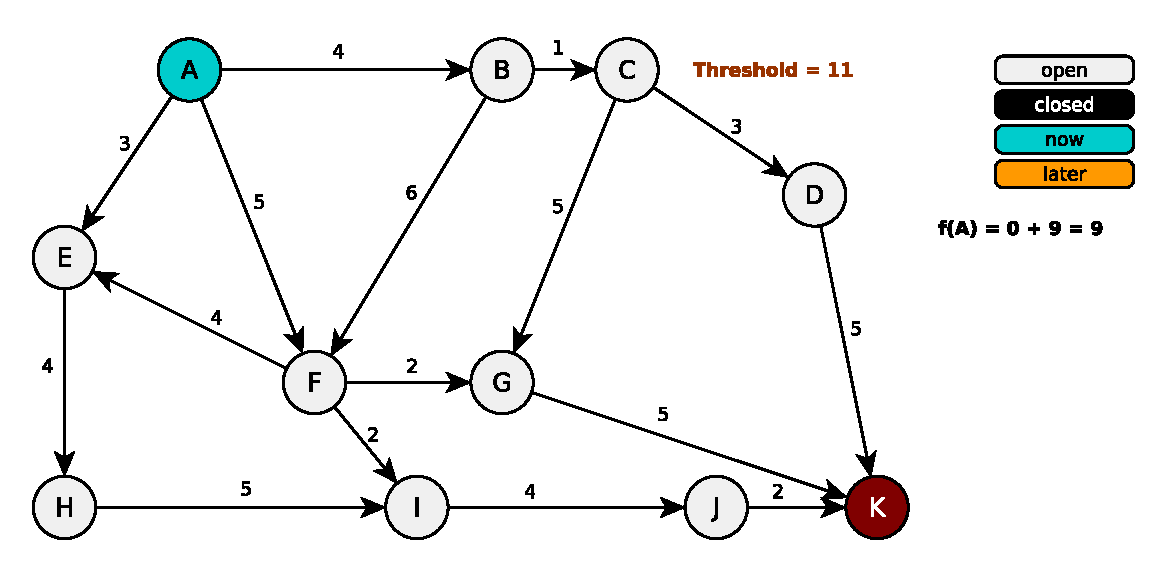
\includegraphics[height=165pt]{fringe1.pdf}
\end{frame}
\begin{frame}
\frametitle{Example 2/7}
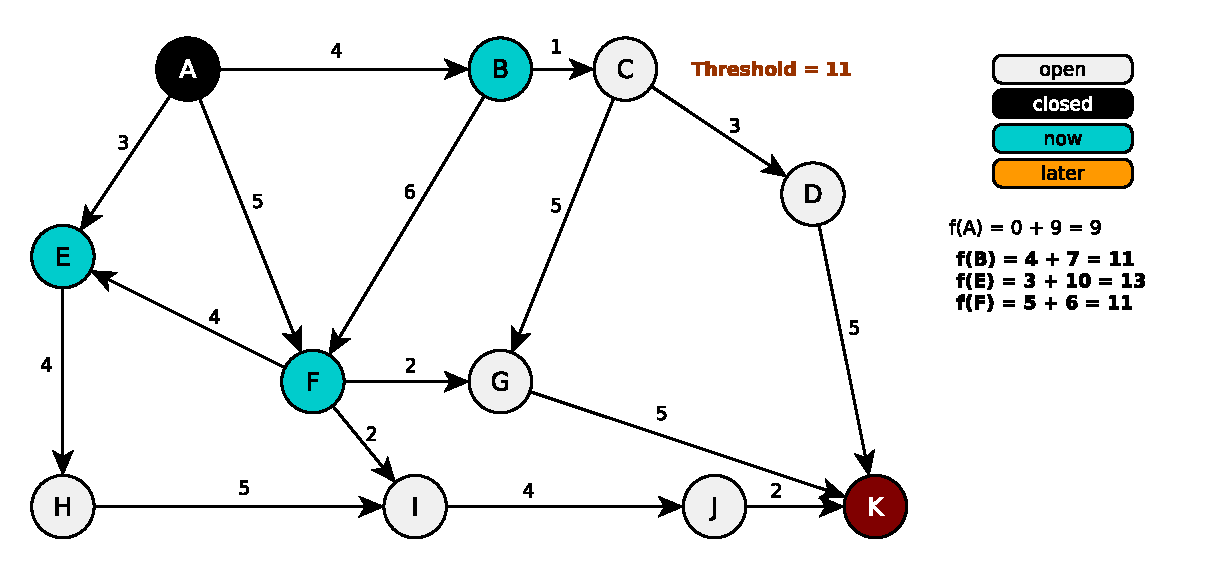
\includegraphics[height=165pt]{fringe2.pdf}
\end{frame}
\begin{frame}
\frametitle{Example 3/7}
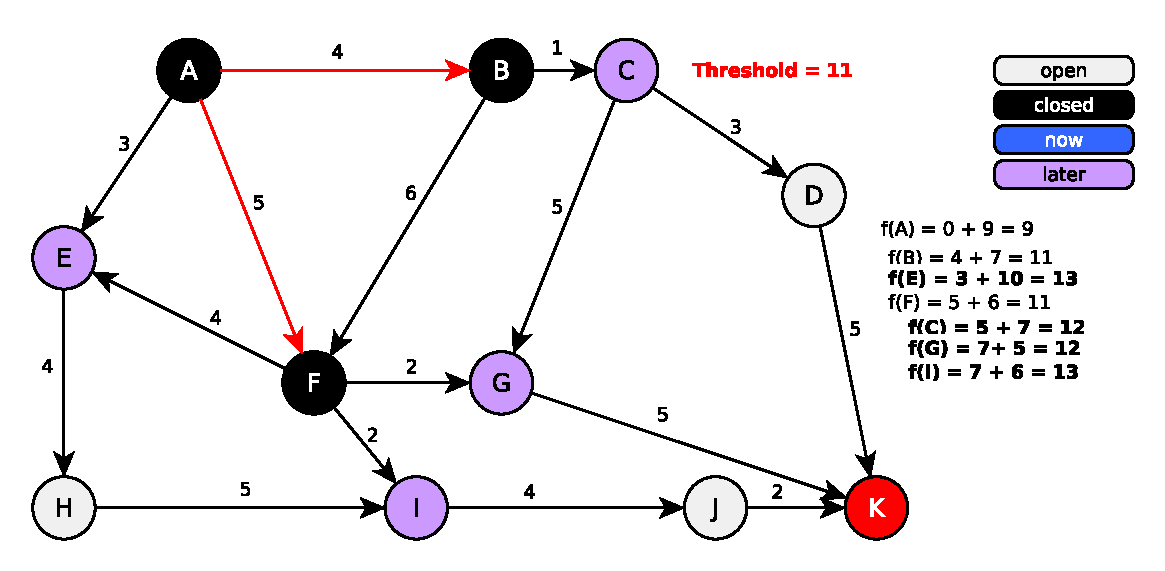
\includegraphics[height=165pt]{fringe3.pdf}
\end{frame}
\begin{frame}
\frametitle{Example 4/7}
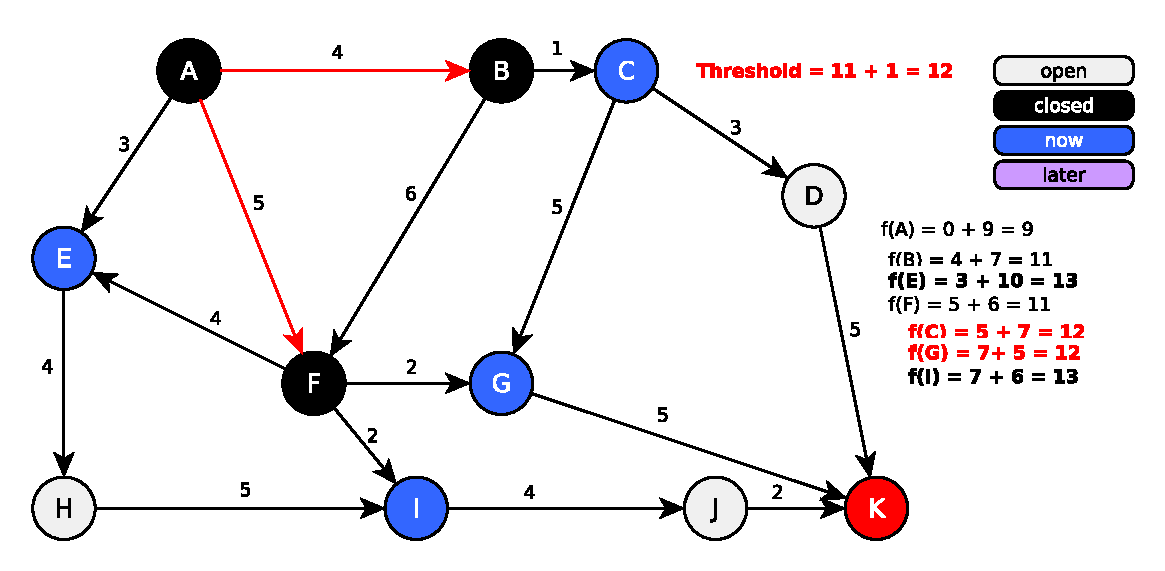
\includegraphics[height=165pt]{fringe4.pdf}
\end{frame}
\begin{frame}
\frametitle{Example 5/7}
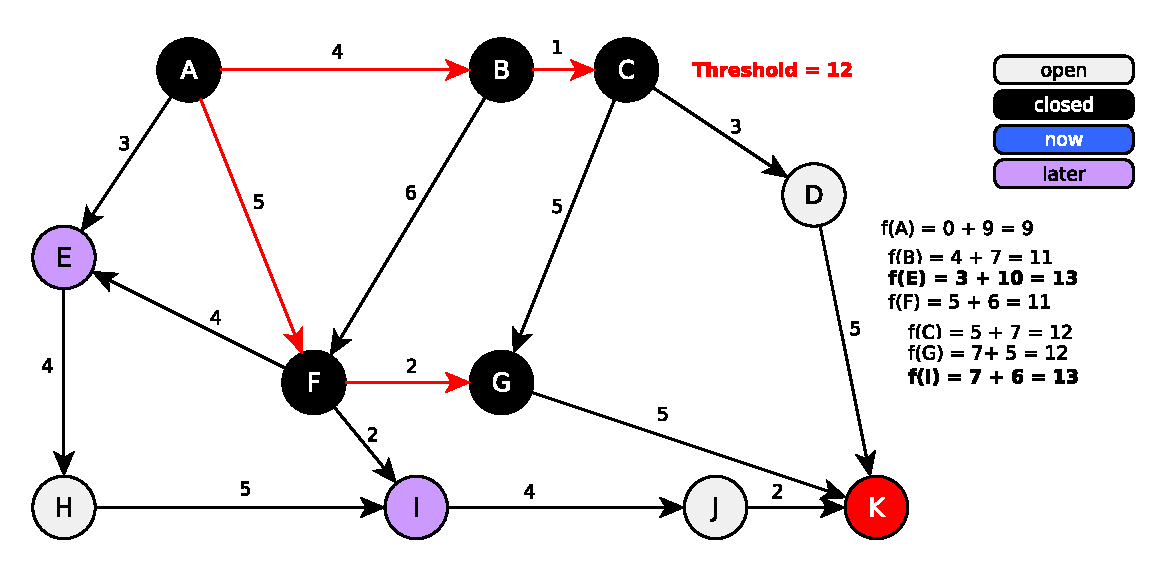
\includegraphics[height=165pt]{fringe5.pdf}
\end{frame}
\begin{frame}
\frametitle{Example 6/7}
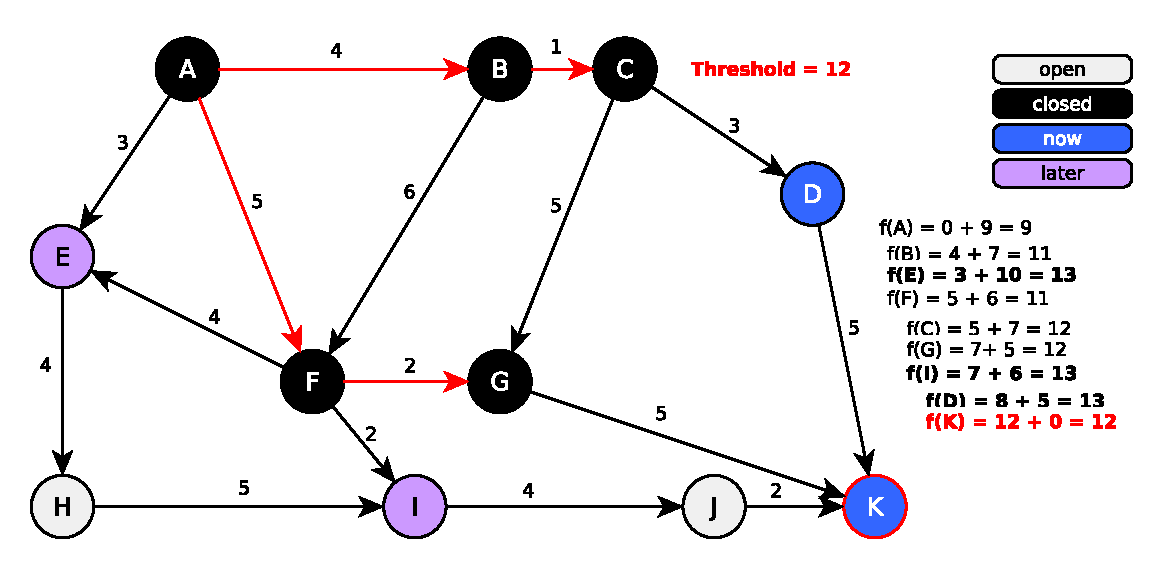
\includegraphics[height=165pt]{fringe6.pdf}
\end{frame}
\begin{frame}
\frametitle{Example 7/7}
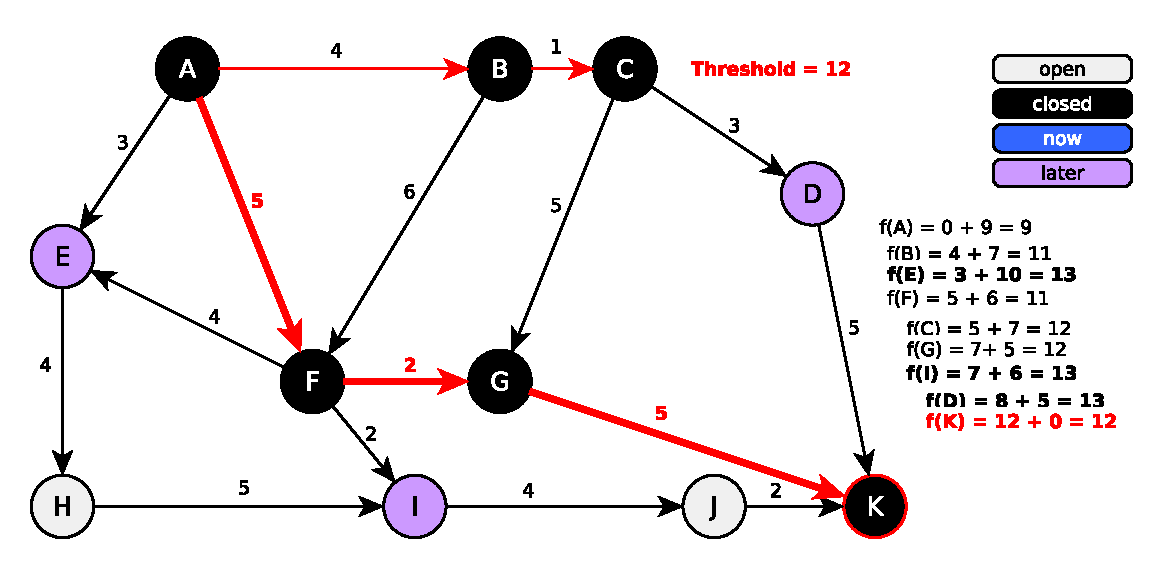
\includegraphics[height=165pt]{fringe7.pdf}
\end{frame}
%------------------------------------------------

%------------------------------------------------

\subsection{Advantages / Disadvantages}

\begin{frame}
\frametitle{Advantages / Disadvantages}
\begin{itemize}
\item Advantages:
	\begin{itemize}
	\item "Best-first" search with no sorting
	\item Fast
	\item Configurable (relaxation function for threshold)
	\end{itemize}
\item Disadvantages:
	\begin{itemize}
	\item Not optimal
	\item Bad configuration may leed to bad path
	\item Worst case not better then A*
	\end{itemize}
\end{itemize}
\end{frame}
%------------------------------------------------



%------------------------------------------------
\section{Implementation and Evaluation}
%------------------------------------------------

\begin{frame}
\frametitle{Implementation and Evaluation}
\begin{itemize}
\item Implementation will be done with MPI
\item Evaluation in terms of
	\begin{itemize}
	\item runtime
	\item length of path compared to optimal path
	\end{itemize}
\item Different configurations for threshold relaxation
\end{itemize}
\end{frame}


%------------------------------------------------
\section{References}
%------------------------------------------------

\begin{frame}
\frametitle{References}
\footnotesize{
\begin{thebibliography}{99} % Beamer does not support BibTeX so references must be inserted manually as below
\bibitem[brand, 2012]{p1} Sandy Brand and Rafael Bidarra (2012)
\newblock Multi-core scalable and efficient pathfinding with
Parallel Ripple Search
\newblock \emph{Computer Animation and Virtual Worlds, Volume 23, Issue 2} 2012, pp 73 -- 85.
\bibitem[brand, 2009]{p1} Sandy Brand (2009)
\newblock Efficient obstacle avoidance using autonomously generated navigation meshes
\newblock \emph{Master Thesis} (Delft University of Technology)
\end{thebibliography}
}
\end{frame}






%------------------------------------------------

\begin{frame}
\Huge{\centerline{The End}}
\end{frame}

%----------------------------------------------------------------------------------------

\end{document} 